\documentclass[tikz,multi=tikzpicture,border=7pt]{standalone}
\usepackage{ctex}
\usepackage{amsmath,amssymb,bm}
\usetikzlibrary{arrows.meta,calc,decorations.pathmorphing,patterns,positioning,angles,quotes,3d}
\tikzset{
  vec/.style={-{Latex[length=2.6mm]},very thick,blue!72!black},
  force/.style={-{Latex[length=2.6mm]},very thick,red!72!black},
  guide/.style={gray!70,dashed},
  body/.style={draw,very thick,fill=blue!8},
  mass/.style={draw,very thick,fill=orange!45,rounded corners=1pt},
  dim/.style={<->,>=Latex,thin},
  ray/.style={-{Latex[length=2.2mm]},thick,orange!80!black},
  wave/.style={blue!70!black,thick}
}
\tikzset{vec/.style={-{Latex[length=2.4mm]},very thick,blue!70!black},force/.style={-{Latex[length=2.4mm]},very thick,red!70!black},impulse/.style={force},ray/.style={-{Latex[length=2.2mm]},thick,orange!80!black},wave/.style={blue!70!black,thick},body/.style={draw,very thick,fill=blue!7},guide/.style={gray!65,dashed},dim/.style={<->,>=Latex,thin},resistor/.style={decorate,decoration={zigzag,segment length=4pt,amplitude=2pt},thick}}
\begin{document}

% 1 question-01
\begin{tikzpicture}[x=1cm,y=1cm,font=\small]

\draw[very thick](-5,-1.34)--(5,1.34);\draw[guide](-5,-1.34)--(-2.8,-1.34);\draw(-4,-1.34)arc(0:15:1)node[midway,right]{$\theta$};
\coordinate(C)at(-.337,1.256);\draw[body](C)circle(1.3);\draw[very thick](C)circle(.48);
\fill(0,0)circle(2pt)node[below]{$P$};\fill(C)circle(2pt)node[left]{$C$};
\draw[very thick](.143,1.256)--(.143,-2.35);\node[mass]at(.143,-2.7){$m$};
\node[align=left]at(3,2.1){初始绳竖直\\轴半径 $r$，轮半径 $R$\\$M=m_1+2m_2$};
\end{tikzpicture}

% 2 solution-01
\begin{tikzpicture}[x=1cm,y=1cm,font=\small]

\begin{scope}[shift={(-3.6,0)}]
\draw[very thick](-2.6,-.7)--(2.6,.7);\coordinate(C)at(-.31,1.159);\draw[body](C)circle(1.2);\fill(0,0)circle(2pt)node[below]{$P$};
\draw[force](C)--++(0,-2)node[below]{$Mg$};\draw[force](0,0)--(-.45,1.68)node[left]{$N$};
\draw[force](0,0)--(1.65,.44)node[right]{$f$（正向）};\draw[force](.15,1.16)--++(-.4,-1.7)node[right]{$T_s$};
\node at(0,-1.7){$Ma=T_s[-\sin(\alpha+\theta)]+f-Mg\sin\theta$};
\end{scope}
\begin{scope}[shift={(3.5,.2)}]
\draw[guide](0,2)--(0,-2);\draw[very thick](0,1.6)--(-.65,-1.5);\draw(0,.6)arc(-90:-102:1)node[left]{$\alpha$};
\draw[vec](0,0)--(1.8,.48)node[right]{$a\bm e_x$};\draw[vec](1.8,.48)--(1.42,-1.2)node[right]{$(r/R)a\bm e_s$};\draw[vec](0,0)--(1.42,-1.2)node[left]{$\bm a_m$};
\node at(0,-2.6){$a\cos(\alpha+\theta)=g\sin\alpha$};\end{scope}
\end{tikzpicture}

% 3 question-02
\begin{tikzpicture}[font=\small,x=1cm,y=1cm]
  \begin{scope}[shift={(-3.8,0)}]
    \draw[very thick] (0,-3.2)--(0,3.4);
    \foreach \y/\name in {2.75/A,1.65/B,.55/C,-.55/D,-1.65/E,-2.75/F}{
      \shade[ball color=orange!55] (0,\y) circle (.28); \node[right] at (.45,\y) {$\name$};}
    \draw[dim] (-.7,1.65)--(-.7,2.75) node[midway,left] {$h$};
    \node at (0,-3.75) {六球碰撞链};
  \end{scope}
  \begin{scope}[shift={(3.4,0)}]
    \draw[very thick] (-2.4,-3.2)--(2.4,-3.2);
    \foreach \y in {-2.45,-1.4,-.35,.7,1.75,2.8}{\shade[ball color=orange!55] (0,\y) circle (.25);}
    \draw[dim] (1.0,-3.2)--(1.0,-2.45) node[midway,right] {$h$};
    \draw[force] (0,3.15)--(0,2.05) node[right] {$g$};
    \node at (0,-3.75) {$N$ 个质点的黏连坠落};
  \end{scope}
\end{tikzpicture}

% 4 solution-02
\begin{tikzpicture}[x=1cm,y=1cm,font=\small]
\begin{scope}[shift={(-4,0)}]\draw[->](-.2,0)--(5,0)node[right]{$t$};\draw[->](0,-.2)--(0,4.7)node[above]{$z_{\rm ff}$};\draw[blue!70!black,thick] plot coordinates {(0.00000,0.20000) (4.50000,4.40000)};
\draw[blue!70!black,thick] plot coordinates {(0.00000,0.60000) (4.50000,3.50000)};
\draw[blue!70!black,thick] plot coordinates {(0.00000,1.20000) (4.50000,2.70000)};
\draw[blue!70!black,thick] plot coordinates {(0.00000,2.10000) (4.50000,1.80000)};
\draw[blue!70!black,thick] plot coordinates {(0.00000,3.40000) (4.50000,1.00000)};
\draw[blue!70!black,thick] plot coordinates {(0.00000,4.40000) (4.50000,0.30000)};

\node[align=center]at(2.2,-1){辅助轨迹穿越；实体球交换速度\\最多 $\binom62=15$ 次};\end{scope}
\begin{scope}[shift={(4,.2)}]\node[mass](K)at(0,1.5){$km$};\draw[body](0,-.5)circle(.2)node[right]{$m$};\draw[vec](0,1.2)--(0,.1)node[right]{$w_k$};\draw[dim](1,-.5)--(1,1.5)node[midway,right]{$h$};
\node[align=center]at(0,-1.6){$u_{k+1}=\dfrac{k}{k+1}\sqrt{u_k^2+2gh}$\\$v_{\rm ground}^2=gh(N+1)(2N+1)/(3N)$};\end{scope}
\end{tikzpicture}

% 5 question-03
\begin{tikzpicture}[x=1cm,y=1cm,font=\small]

\draw[->](-2,0)--(2.8,0)node[right]{切向};\draw[->](0,-2.5)--(0,2.4)node[above]{径向向外};
\fill[blue!60](0,0)circle(3pt)node[above left]{地球、彗星相遇处};\draw[vec](0,0)--(2.25,0)node[below]{$v_E=2\pi$};
\draw[vec](0,0)--(.9,-2.3)node[right]{$\bm v_c$（接近太阳）};\draw[guide](0,0)--(0,-3);\fill[orange!80](0,-3)circle(3pt)node[below]{太阳方向};
\node[align=left,anchor=west]at(4,.2){$T=1200$ 年，$a=T^{2/3}$ AU\\$r_1=0.1$ AU，$r_2=2a-r_1$\\在 $r=1$ AU 处取入境支\\$v_t>0,\quad v_r<0$};
\end{tikzpicture}

% 6 solution-03
\begin{tikzpicture}[x=1cm,y=1cm,font=\small]

\begin{scope}[shift={(-3.7,0)}]\draw[->](-2.5,0)--(2.5,0)node[right]{$X$（地球运动方向）};\draw[->](0,-3)--(0,1.3)node[above]{$Y$（向外）};
\draw[vec](0,0)--(1.1,-2.7)node[right]{$\bm v_c$};\draw[vec](0,0)--(2.45,0)node[above]{$\bm v_E$};\draw[vec,red!70!black](2.45,0)--(1.1,-2.7)node[midway,left]{$\bm v_{c/E}$};
\node at(0,-3.8){$v_{c/E}=9.1$ AU/年};\end{scope}
\begin{scope}[shift={(3.8,-.2)}]\draw[->](-2.5,0)--(2.5,0)node[right]{$u_X$};\draw[->](0,-2.8)--(0,1.2)node[above]{$u_Y$};
\fill(-.8,-2.5)circle(2pt)node[right]{$\bm u_0$};\draw[vec](-.8,-2.5)--(-1.8,-.2)node[midway,left]{$-s\hat{\bm d}$};\fill(-1.8,-.2)circle(2pt)node[above]{$\bm u_{\rm small}$};
\draw[guide](-2.2,-.8)..controls(-1.7,-.2)and(-1,.4)..(-.3,.8);\node[align=center]at(0,-3.8){临界双曲线近地点 $r_p=R_E$\\只沿彗星日心切向改变速度\\$s_{\min}=4.0062\times10^4$ m/s};\end{scope}
\end{tikzpicture}

% 7 question-04
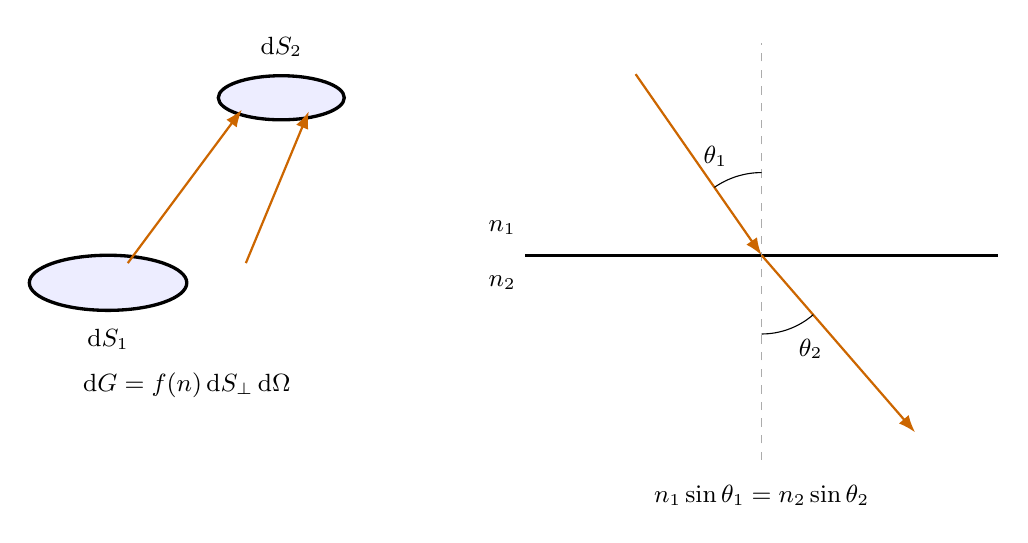
\begin{tikzpicture}[font=\small,x=1cm,y=1cm]
  \begin{scope}[shift={(-3.7,0)}]
    \draw[body] (-1.0,-.35) ellipse (1.0 and .35) node[below=.45cm] {$\mathrm dS_1$};
    \draw[body] (1.2,2.0) ellipse (.8 and .28) node[above=.38cm] {$\mathrm dS_2$};
    \draw[ray] (-.75,-.1)--(.7,1.85); \draw[ray] (.75,-.1)--(1.55,1.83);
    \node at (0,-1.65) {$\mathrm dG=f(n)\,\mathrm dS_\perp\,\mathrm d\Omega$};
  \end{scope}
  \begin{scope}[shift={(3.6,0)}]
    \draw[very thick] (-3,0)--(3,0); \node[left] at (-3,.35) {$n_1$}; \node[left] at (-3,-.35) {$n_2$};
    \draw[guide] (0,-2.6)--(0,2.7);
    \draw[ray] (-1.6,2.3)--(0,0); \draw[ray] (0,0)--(1.95,-2.25);
    \draw (0,1.05) arc (90:124.8:1.05) node[midway,above left] {$\theta_1$};
    \draw (0,-1.0) arc (-90:-49:1.0) node[midway,below right] {$\theta_2$};
    \node at (0,-3.05) {$n_1\sin\theta_1=n_2\sin\theta_2$};
  \end{scope}
\end{tikzpicture}

% 8 solution-04
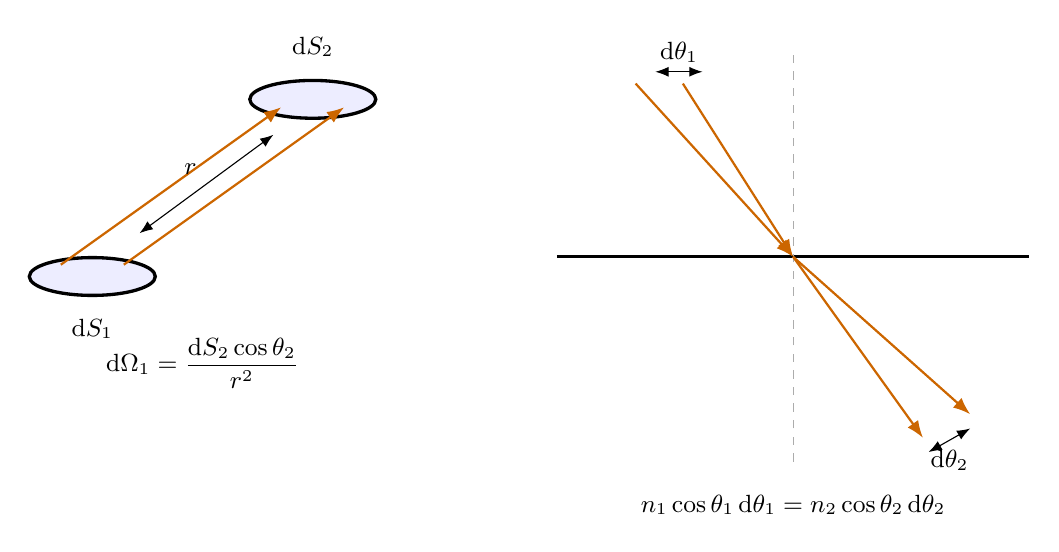
\begin{tikzpicture}[font=\small,x=1cm,y=1cm]
  \begin{scope}[shift={(-3.8,0)}]
    \draw[body] (-1.4,-.25) ellipse (.8 and .24) node[below=.4cm] {$\mathrm dS_1$};
    \draw[body] (1.4,2.0) ellipse (.8 and .24) node[above=.4cm] {$\mathrm dS_2$};
    \draw[ray] (-1.8,-.1)--(1.0,1.9); \draw[ray] (-1.0,-.1)--(1.8,1.9);
    \draw[dim] (-.8,.3)--(.9,1.55) node[midway,above left] {$r$};
    \node at (0,-1.35) {$\mathrm d\Omega_1=\dfrac{\mathrm dS_2\cos\theta_2}{r^2}$};
  \end{scope}
  \begin{scope}[shift={(3.7,0)}]
    \draw[very thick] (-3,0)--(3,0); \draw[guide] (0,-2.6)--(0,2.6);
    \draw[ray] (-2.0,2.2)--(0,0); \draw[ray] (-1.4,2.2)--(0,0);
    \draw[ray] (0,0)--(1.65,-2.3); \draw[ray] (0,0)--(2.25,-2.0);
    \draw[dim] (-1.75,2.35)--(-1.15,2.35) node[midway,above] {$\mathrm d\theta_1$};
    \draw[dim] (1.72,-2.48)--(2.25,-2.18) node[midway,below] {$\mathrm d\theta_2$};
    \node at (0,-3.15) {$n_1\cos\theta_1\,\mathrm d\theta_1=n_2\cos\theta_2\,\mathrm d\theta_2$};
  \end{scope}
\end{tikzpicture}

% 9 question-05
\begin{tikzpicture}[x=1cm,y=1cm,font=\small]

\draw[->](-4.5,0)--(4.8,0)node[right]{$x$};\draw[very thick](0,0)ellipse(.55 and 1.6);\node at(0,-2.1){闭合无电阻环，$L$};
\node[mass]at(3,0){$S\quad N$};\draw[vec](3,.75)--(4.3,.75)node[right]{$\bm m$};\draw[vec](3,-.7)--(1.5,-.7)node[left]{$v_0$};\draw[dim](0,2.1)--(3,2.1)node[midway,above]{$x>0$};
\end{tikzpicture}

% 10 solution-05
\begin{tikzpicture}[font=\small,x=1cm,y=1cm]
  \begin{scope}[shift={(-3.8,.25)}]
    \fill (0,0) circle (2.5pt) node[left] {磁极 $q_m$};
    \begin{scope}[shift={(2.7,0)},xscale=.35]\draw[very thick] (0,0) circle (1.7);\end{scope}
    \draw[ray] (0,0)--(2.7,1.7); \draw[ray] (0,0)--(2.7,-1.7);
    \draw (1.0,0) arc (0:32:1.0) node[midway,right] {$\vartheta$};
    \draw[dim] (0,-2.25)--(2.7,-2.25) node[midway,below] {$x$};
    \node at (0,-3.0) {$\Omega=2\pi(1-\cos\vartheta)$};
  \end{scope}
  \begin{scope}[shift={(3.7,0)}]
    \draw[->] (-2.9,0)--(3.0,0) node[right] {$x$}; \draw[->] (0,-.3)--(0,3.0) node[above] {$U$};
    \draw[very thick,blue!65,domain=-2.7:2.7,samples=100] plot (\x,{2.35/(1+0.55*\x*\x)^3});
    \draw[guide] (-2.8,2.35)--(2.8,2.35) node[right] {$U(0)$};
    \node at (0,-1.0) {$U(x)=\dfrac{\Phi^2(x)}{2L}$};
    \draw[vec] (2.0,.4)--(.8,.4) node[midway,below] {$v_0$};
  \end{scope}
\end{tikzpicture}

% 11 question-06
\begin{tikzpicture}[x=1cm,y=1cm,font=\small]

\node[draw,align=center](S)at(-4.8,0){发射端\\正交线偏振交替};\node[draw,align=center](W)at(-1.5,0){可调四分之一波片\\快轴 $45^\circ$};\node[draw,align=center](M)at(2,0){反射镜};
\draw[ray](S)--(W);\draw[ray](W)--(M);\draw[ray](M.south)--(2,-1.7)--(-.5,-1.7);
\node[draw,align=center](R)at(-2.1,-1.7){接收固定波片\\与正交检偏片};\draw[ray](-.5,-1.7)--(R);
\node at(0,1.4){各色发射波片调到 $\delta=\pi/2$；接收波片固定};
\end{tikzpicture}

% 12 solution-06
\begin{tikzpicture}[x=1cm,y=1cm,font=\small]

\begin{scope}[shift={(-3.5,0)}]\draw[->](-2,0)--(2.2,0)node[right]{$x$};\draw[->](0,-2)--(0,2.2)node[above]{$y$};\draw[very thick](0,0)circle(1.4);
\foreach\a/\lab in{0/0,90/{T/4},180/{T/2},270/{3T/4}}{\draw[vec](0,0)--({1.4*cos(\a)},{1.4*sin(\a)});\node at({1.9*cos(\a)},{1.9*sin(\a)}){$\lab$};}
\draw[force](1.4,0)arc(0:65:1.4);\node[align=center]at(0,-3){$e^{-i\omega t}$ 约定；电矢量随时间逆时针\\手性还须声明观察方向};\end{scope}
\begin{scope}[shift={(3.6,0)}]\draw[very thick](0,0)ellipse(1.55 and 1.15);\draw[->](-2.2,0)--(2.2,0)node[right]{$E_x$};\draw[->](0,-1.8)--(0,2)node[above]{$E_y$};
\node[align=center]at(0,-2.7){相位误差 $\varepsilon=\delta-\pi/2$\\$I_{\rm ghost}/I_{\rm normal}=\tan^2(\varepsilon/2)$\\小误差：$\simeq\varepsilon^2/4$};\end{scope}
\end{tikzpicture}

% 13 question-07
\begin{tikzpicture}[font=\small,x={(1cm,0cm)},y={(.55cm,.28cm)},z={(0cm,1cm)}]
  \draw[very thick] (0,0,-2.2)--(0,0,2.2); \draw[very thick] (7,0,-2.2)--(7,0,2.2);
  \draw[very thick] (0,0,2.2) arc (90:450:1 and 2.2); \draw[very thick] (7,0,2.2) arc (90:450:1 and 2.2);
  \draw[very thick] (0,0,2.2)--(7,0,2.2) (0,0,-2.2)--(7,0,-2.2);
  \foreach \s in {1.2,2.3,3.4,4.5,5.6}{
    \draw[blue!65,thick] (\s-.65,0,2.05) .. controls (\s+.5,1.1,1.0) and (\s+.5,-1.1,-1.0) .. (\s-.65,0,-2.05)
      .. controls (\s-1.45,-1.1,-1.0) and (\s-1.45,1.1,1.0) .. cycle;}
  \draw[->] (0,0,0)--(8,0,0) node[right] {$z$};
  \draw[force] (3.4,0,2.05)--(4.35,0,1.8) node[right] {$I$};
  \node at (3.5,0,-3.0) {圆柱面上的倾斜椭圆匝};
\end{tikzpicture}

% 14 solution-07
\begin{tikzpicture}[x=1cm,y=1cm,font=\small]

\begin{scope}[shift={(-3.5,0)}]\draw[very thick](0,0)circle(1.7);\draw[->](-2.4,0)--(2.5,0)node[right]{$x$};\draw[->](0,-2.3)--(0,2.4)node[above]{$y$};
\foreach\a in{30,75,120,150}{\node at({1.7*cos(\a)},{1.7*sin(\a)}){$\odot$};}\foreach\a in{210,255,300,330}{\node at({1.7*cos(\a)},{1.7*sin(\a)}){$\otimes$};}
\draw[vec](-.9,0)--(.9,0)node[below]{$\bm B_\perp$};\node[align=center]at(0,-3){$K_z=nI\tan\theta\sin\varphi$\\$\odot$：$+z$；$\otimes$：$-z$};\end{scope}\begin{scope}[shift={(3.5,0)}]\draw[very thick](0,0)circle(1);\draw[vec,thin] (-2.000,-2.000)--++(0.000,0.043);
\draw[vec,thin] (-2.000,-1.300)--++(0.024,0.055);
\draw[vec,thin] (-2.000,0.000)--++(0.085,-0.000);
\draw[vec,thin] (-2.000,1.300)--++(0.024,-0.055);
\draw[vec,thin] (-2.000,2.000)--++(0.000,-0.043);
\draw[vec,thin] (-1.300,-2.000)--++(-0.024,0.055);
\draw[vec,thin] (-1.300,-1.300)--++(0.000,0.101);
\draw[vec,thin] (-1.300,0.000)--++(0.201,-0.000);
\draw[vec,thin] (-1.300,1.300)--++(0.000,-0.101);
\draw[vec,thin] (-1.300,2.000)--++(-0.024,-0.055);
\draw[vec,thin] (0.000,-2.000)--++(-0.085,-0.000);
\draw[vec,thin] (0.000,-1.300)--++(-0.201,-0.000);
\draw[vec,thin] (0.000,1.300)--++(-0.201,0.000);
\draw[vec,thin] (0.000,2.000)--++(-0.085,0.000);
\draw[vec,thin] (1.300,-2.000)--++(-0.024,-0.055);
\draw[vec,thin] (1.300,-1.300)--++(0.000,-0.101);
\draw[vec,thin] (1.300,0.000)--++(0.201,0.000);
\draw[vec,thin] (1.300,1.300)--++(0.000,0.101);
\draw[vec,thin] (1.300,2.000)--++(-0.024,0.055);
\draw[vec,thin] (2.000,-2.000)--++(0.000,-0.043);
\draw[vec,thin] (2.000,-1.300)--++(0.024,-0.055);
\draw[vec,thin] (2.000,0.000)--++(0.085,0.000);
\draw[vec,thin] (2.000,1.300)--++(0.024,0.055);
\draw[vec,thin] (2.000,2.000)--++(0.000,0.043);

\draw[vec](-.65,0)--(.65,0);\node[align=center]at(0,-3){横截面外场按 $\rho^{-2}$ 衰减\\内部横场均匀；$B_z=\mu_0nI$};\end{scope}
\end{tikzpicture}

% 15 question-08
\begin{tikzpicture}[font=\small,x=1cm,y=1cm]
  \draw[very thick,gray!65,dashed] (0,0) ellipse (3.2 and 1.2);
  \draw[very thick,blue!65] (0,0) ellipse (4.5 and 1.7);
  \shade[ball color=black!88] (0,0) circle (1.45);
  \filldraw[fill=orange!60] (3.9,.85) circle (.18) node[above right] {质点};
  \draw[vec] (3.9,.85)--++(-.55,1.25) node[above] {$\bm v$};
  \draw[dim] (0,-2.4)--(4.15,-2.4) node[midway,below] {$r$};
  \node at (0,2.45) {史瓦西黑洞赤道面内的圆轨道};
\end{tikzpicture}

% 16 solution-08
\begin{tikzpicture}[x=1cm,y=1cm,font=\small]
\begin{scope}[shift={(-4,0)}]\draw[->](.4,-1)--(5.8,-1)node[right]{$r/\mu$};\draw[->](.5,-1)--(.5,2.5)node[above]{$V_{\rm eff}$};\draw[very thick,blue!70!black] plot coordinates {(0.67500,-0.11722) (0.70738,0.39050) (0.73977,0.76359) (0.77215,1.03613) (0.80453,1.23314) (0.83691,1.37313) (0.86930,1.46997) (0.90168,1.53406) (0.93406,1.57332) (0.96644,1.59376) (0.99883,1.59999) (1.03121,1.59556) (1.06359,1.58320) (1.09597,1.56502) (1.12836,1.54266) (1.16074,1.51740) (1.19312,1.49021) (1.22550,1.46186) (1.25789,1.43293) (1.29027,1.40388) (1.32265,1.37504) (1.35503,1.34669) (1.38742,1.31900) (1.41980,1.29213) (1.45218,1.26616) (1.48456,1.24118) (1.51695,1.21722) (1.54933,1.19430) (1.58171,1.17243) (1.61409,1.15161) (1.64648,1.13182) (1.67886,1.11305) (1.71124,1.09526) (1.74362,1.07842) (1.77601,1.06251) (1.80839,1.04750) (1.84077,1.03333) (1.87315,1.02000) (1.90554,1.00744) (1.93792,0.99564) (1.97030,0.98456) (2.00268,0.97416) (2.03507,0.96442) (2.06745,0.95530) (2.09983,0.94677) (2.13221,0.93880) (2.16460,0.93136) (2.19698,0.92444) (2.22936,0.91799) (2.26174,0.91201) (2.29413,0.90646) (2.32651,0.90132) (2.35889,0.89658) (2.39128,0.89221) (2.42366,0.88818) (2.45604,0.88450) (2.48842,0.88113) (2.52081,0.87806) (2.55319,0.87528) (2.58557,0.87277) (2.61795,0.87052) (2.65034,0.86850) (2.68272,0.86672) (2.71510,0.86516) (2.74748,0.86381) (2.77987,0.86265) (2.81225,0.86168) (2.84463,0.86089) (2.87701,0.86026) (2.90940,0.85979) (2.94178,0.85948) (2.97416,0.85930) (3.00654,0.85926) (3.03893,0.85935) (3.07131,0.85956) (3.10369,0.85989) (3.13607,0.86032) (3.16846,0.86086) (3.20084,0.86149) (3.23322,0.86222) (3.26560,0.86303) (3.29799,0.86393) (3.33037,0.86491) (3.36275,0.86596) (3.39513,0.86708) (3.42752,0.86826) (3.45990,0.86951) (3.49228,0.87082) (3.52466,0.87218) (3.55705,0.87360) (3.58943,0.87506) (3.62181,0.87657) (3.65419,0.87813) (3.68658,0.87972) (3.71896,0.88136) (3.75134,0.88303) (3.78372,0.88474) (3.81611,0.88648) (3.84849,0.88825) (3.88087,0.89005) (3.91326,0.89187) (3.94564,0.89372) (3.97802,0.89559) (4.01040,0.89749) (4.04279,0.89940) (4.07517,0.90133) (4.10755,0.90328) (4.13993,0.90525) (4.17232,0.90723) (4.20470,0.90922) (4.23708,0.91123) (4.26946,0.91324) (4.30185,0.91527) (4.33423,0.91731) (4.36661,0.91935) (4.39899,0.92140) (4.43138,0.92346) (4.46376,0.92553) (4.49614,0.92760) (4.52852,0.92967) (4.56091,0.93175) (4.59329,0.93383) (4.62567,0.93592) (4.65805,0.93800) (4.69044,0.94009) (4.72282,0.94218) (4.75520,0.94426) (4.78758,0.94635) (4.81997,0.94844) (4.85235,0.95052) (4.88473,0.95260) (4.91711,0.95469) (4.94950,0.95676) (4.98188,0.95884) (5.01426,0.96091) (5.04664,0.96298) (5.07903,0.96505) (5.11141,0.96711) (5.14379,0.96917) (5.17617,0.97122) (5.20856,0.97326) (5.24094,0.97531) (5.27332,0.97734) (5.30570,0.97938) (5.33809,0.98140) (5.37047,0.98342) (5.40285,0.98543) (5.43523,0.98744) (5.46762,0.98944) (5.50000,0.99144)};

\draw[guide](1,-1)--(1,1.6)node[above]{$r_-=4\mu$};\draw[guide](3,-1)--(3,.859)node[below]{$r_+=12\mu$};\node at(2.7,-2){示例 $L=4GMm_0/c$；稳定支 $r_+>6\mu$};\end{scope}
\begin{scope}[shift={(4,0)}]\fill[black!80](0,0)circle(.45);\draw[very thick](0,0)circle(1.2);\fill(1.2,0)circle(2pt);
\draw[ray](1.2,0)..controls(1.2,1.1)and(.6,2.1)..(-1.7,3.1);\draw[guide](-2.8,3.6)--(1.7,1.5);
\draw[dim](0,0)--(.879,1.884)node[midway,right]{$b$（渐近线垂距）};\draw[dim](0,-.3)--(1.2,-.3)node[midway,below]{$6\mu$};
\node[align=center]at(0,-2){光路示意；$\mu=GM/c^2$\\$b=3\sqrt6\mu,\quad\nu_\infty=\sqrt2\nu$};\end{scope}
\end{tikzpicture}

\end{document}
